\chapter{Generalized Linear Models}
\label{cha:glm}

\section{Introduction}
\label{sec:glm-introduction}
In this chapter we will explain the concepts of generalized linear models\cite{caltechmachinelearning}\cite{wikiglm}. This term indicates a generalization of simple linear regression that allows for a wide range of output variables. First we will go over the basics of linear models, gradually building up to the definition of generalized linear models. Next, we will describe what actual data looks like and how a model is computed from it. After that we will tackle the more recent innovation of regularization that will greatly improve our previous models by exploiting the bias-variance trade-off to reduce overfitting. Lastly we will outline the validation method that will be used to test the performance of the models.

\section{Classical linear models}
\label{sec:glm-classicallinearmodels}
When we think of classical linear models, we can imagine a set of numeric explanatory (or input) variables and a numerical dependent (or output) variable. By making a linear combination of the explanatory variables we attempt to estimate a value for the dependent variable. Depending on the type of dependent variable the linear method gets a different name. In the following sections we will outline several of them.

\subsection{Linear Regression}
\label{subsec:glm-linear-regression}
The simplest version of a linear model is called linear regression\cite{caltechmachinelearning}\cite{wikilinearregression}. In this case the input variables are combined using a linear combination, and the result of this calculation is immediately used as the final estimate. Imagine we have a dataset of size N where each sample has M explanatory variables. Then we can write linear regression as:\\
\begin{equation}
\begin{split}
y_{n} = \sum_{i=1}^{M}w_{i}x_{in} = \bm{w^{T}x}   \qquad for\ n=1..N
\end{split}
\end{equation}
where
\begin{itemize}
	\item $y_{n}$ is the output for sample $n$
	\item $w_{i}$ is the model parameter (coefficient) for explanatory variable $i$
	\item $x_{in}$ is the value for explanatory variable $i$ for sample $n$
	\item $\bm{w^{T}x}$ is the vector notation for the inner product of $\bm{w}$ and $\bm{x}$
\end{itemize}
For the other linear methods we will define a function each time that is applied to the result of the linear combination. We could do the same for linear regression and say that the applied function is the identity function. A schema for this computation is shown on figure \ref{fig:glm-linear-regression}.\\
\begin{figure}
	\centering
	\includegraphics[scale=.6]{images/linear_regression.png}
	\caption{Schema for linear regression}
	\label{fig:glm-linear-regression}
\end{figure}
\subsection{Linear Classification}
\label{subsec:glm-linear-classification}
The next method is called linear classification\cite{caltechmachinelearning}\cite{wikiclassification}. The difference with linear regression is that we have a different type of output variable. In a classification task we want to predict a class from a list of potential classes. For instance, we could try to predict whether tomorrow will be a sunny day or not. Notice that there are only 2 possible outcomes: 'sunny' or 'not sunny' and we could represent these outcomes as 0 and 1 in our model. This form would be called binary classification because we have 2 possible classes. It is very easy to extend this method to multi-class classification.\\
The computation in this method starts out exactly the same, combining the input variables using a linear combination. Next, we have to define a threshold to indicate which examples belong to one class or another. In the case of binary classification we would define 1 threshold, and if the result of the linear combination is higher than the threshold we would predict one class. If it is lower, we would predict the other class. The function used here would be called a sign function, which maps real values onto one of 2 possible outcomes. We could represent this computation with the following formula: 
\begin{equation}
\begin{split}
y_{n} =
\begin{cases} 
0 & if\ \bm{w^{T}x} \leq t \\
1 & if\ \bm{w^{T}x} > t 
\end{cases}
\qquad for\ n=1..N
\end{split}
\end{equation}
where
\begin{itemize}
	\item $y_{n}$ is the output for sample $n$
	\item $\bm{w^{T}x}$ is the vector notation for the inner product of $\bm{w}$ and $\bm{x}$
	\item $t$ is the classification threshold
\end{itemize}
A schema for this computation is shown on figure \ref{fig:glm-linear-classification}.
\begin{figure}
	\centering
	\includegraphics[scale=.6]{images/linear_classification.png}
	\caption{Schema for linear classification}
	\label{fig:glm-linear-classification}
\end{figure}
\subsection{Logistic Regression}
\label{subsec:glm-logistic-regression}
The third method we want to present is called logistic regression\cite{caltechmachinelearning}\cite{wikilogistic}. In this case, the output variable we want to predict comes from a binomial distribution. This means that they are the result of a probabilistic event. An example would be tossing a coin and checking whether the result is heads or tails. While the outcome is binary (heads or tails) we know that there is an underlying probability for the coin to be heads or tails, and we would like to know this probability. \\
The idea is still the same. We will make a linear combination of the input variables. However this time we will use a logistic function to produce our estimate. The logistic function is a function that maps real numbers onto the range $[0,1]$. This result can then be interpreted as an estimate for the probability. We could represent logistic regression mathematically as:
\begin{equation}
\begin{split}
y_{n} = \theta(\sum_{i=1}^{M}w_{i}x_{in})= \theta(\bm{w^{T}x}) \qquad for\ n=1..N
\end{split}
\end{equation}
where
\begin{itemize}
	\item $y_{n}$ is the output for sample $n$
	\item $w_{i}$ is the model parameter (coefficient) for explanatory variable $i$
	\item $x_{in}$ is the value for explanatory variable $i$ for sample $n$
	\item $\bm{w^{T}x}$ is the vector notation for the inner product of $\bm{w}$ and $\bm{x}$
	\item $\theta(x)$ is a logistic function, also called a sigmoid function. An example sigmoid function is $\frac{e^{x}}{1+e^{x}}$
\end{itemize}
\begin{figure}
	\centering
	\includegraphics[scale=.6]{images/logistic_regression.png}
	\caption{Schema for logistic regression}
	\label{fig:glm-logistic-regression}
\end{figure}
A schema for this computation is shown on figure \ref{fig:glm-logistic-regression}.
The logistic regression method is the one that will be most widely used throughout this thesis.

\section{Training a model}
\label{sec:glm-trainingamodel}
In order to understand the integration strategies that will be explained later on, it is useful to know how exactly the models come to be. This section will explain what the input data for our linear models actually looks like, and how we get from this data to a model that we can use for future predictions.
\subsection{The data}

The data we use consists of two parts: the input data, which can be seen as a matrix where the columns are the explanatory variables and each row is an example. And secondly the output data, which can be seen as a vector where each value indicates the value of the dependent variable for a single example. \\
It is easy to see that the length of the output vector has to be equal to the amount of rows in the input matrix, indeed there should be one output value for each example. This amount is often called the size of the dataset and we would like it to be as big as possible. Especially when we are dealing with a large number of explanatory variables, it is essential to have a reasonable amount of examples aswell. This will be discussed in more detail in section \ref{sec:glm-overfitting} on overfitting. 

\subsection{Gradient descent}
In this section we will explain how we get from the input data to the model\cite{caltechmachinelearning}\cite{wikigd}\cite{gradientdescentvariants}. The idea here is that we have some error measure. The error measure is a sort of rating for our current model as it indicates how big the mistakes are that our current model makes. Once we have a way of computing this error, we can try to minimize the error to obtain our 'best' possible model.
\subsubsection{Error measure}
In logistic regression the error measure we use is called the cross-entropy error\cite{caltechmachinelearning}. The formula for this error is the following:
$$
	E_{in}(w) = \frac{1}{N}\sum_{n=1}^{N}ln(1+e^{-y_{n}w^{T}x_{n}})
$$
where
\begin{itemize}
	\item $x_{n}$ is the vector of values for the explanatory variables for example $n$.
	\item $y_{n}$ is the value of the dependent variable for example $n$.
	\item $w^T$ is the transpose of the weights vector. These are the parameters of our model that we can adjust.
	\item $N$ is the size of our dataset.
	\item $E_{in}(w)$ is the in-sample error. This is the cross-entropy error that we make on the examples in our dataset. It is a function of the weights $w$.
\end{itemize}
We can intuitively see that this is a reasonable error measure. It is an averaged sum over all examples, where for each example we compute an individual error made on that example. Notice that $w^{T}x_{n}$ is the linear combination of the input variables that our current model suggests. This is the prediction that our current model would make for example $n$ and is a real valued number. On the other hand $y_{n}$ is the actual correct prediction for example $n$ and has a value of 0 or 1. If the signs of $w^{T}x_{n}$ and $y_{n}$ agree then our current model actually makes a correct prediction for this example. We can see that in this case the exponential becomes close to 0, making our error for example $n$ very small, as we would expect. If however their signs are opposite, the exponential becomes larger as our incorrect prediction becomes larger. This in turn will increase the error, again as we would expect. Thus we can see that if we were to minimize this error, we are moving towards a model that tries to make correct predictions.
\subsubsection{The gradient descent method}
When trying to minimize a function, a general approach would be to try and compute the derivative of the function, and find the value where this derivative equals zero. In the case of linear regression it is actually possible to compute this minimum in one step. More details about this can be found in appendix //TODO ADD AND REFERENCE APPENDIX. \\
In the case of logistic regression however it is not possible to find an analytic solution to this problem. The best we can do is put ourselves somewhere on the error surface and try to move towards the minimum in small steps. This is called an iterative approach. Remember that our error function looks like this:
$$
E_{in}(w) = \frac{1}{N}\sum_{n=1}^{N}ln(1+e^{-y_{n}w^{T}x_{n}})
$$
We can now compute its derivative with respect to $w$:
$$
\nabla E_{in}(w) = -\frac{1}{N}\sum_{n=1}^{N}\frac{y_{n}x_{n}}{1+e^{y_{n}w^{T}x_{n}}}
$$
The problem is to find the set of weights $w$ for which the derivative becomes 0 (or that minimizes the error). We can start out with an initial set of weights $w(0)$ and then iteratively update these weights so we move towards the minimum. Let's call the direction in which we update our weights $v$. The update we make to $w$ then becomes:
$$
w(t+1) = w(t) + \eta v
$$
where
\begin{itemize}
	\item $w(t+1)$ are the updated weights for this iteration.
	\item $w(t)$ are the current weights before we make a move.
	\item $v$ is a unit vector pointing in the direction we want to move.
	\item $\eta$ is a number that indicates how big the move is that we make, also called the step size.
\end{itemize}
Remember that the gradient of a function at a certain point always points towards the steepest slope upwards\cite{gradientdirection}\cite{gradientdirection2}. In our case we would like to find the minimum, so it is a good idea to move our weights in the direction of steepest descent. The direction $v$ that we are moving towards then becomes the normalized opposite direction of the gradient:
$$
v = -\frac{\nabla E_{in}(w(t))}{\lVert\nabla E_{in}(w(t))\rVert}
$$
We can now summarize the gradient descent method as follows: \\ \\
\begin{algorithm}[H]
	\KwData{x, y}
	initialize weights w(0) \\
	\While{Stopcondition is not met}{
		Compute gradient $\nabla E_{in}(w(t))$\\
		Compute update direction $v$ \\
		Update weights $w(t+1) = w(t) + \eta v$
	}
\caption{Gradient Descent algorithm}
\end{algorithm}

There are two non-trivial issues in this computation: the initialization of the weights and the stopcondition. \\ \\
Weight initialization is sometimes a very tricky thing to do, in the case of logistic regression however it is acceptable to set $w(0)$ equal to the zero-vector as this corresponds to no correlation between any of the input variables and the output variable, and the result of the sigmoid function would be 0.5 or 50\% meaning the model has no preference for either outcome.\\ \\
The stopcondition however is a bigger issue and usually the way to go here is to make a combination of several stop criteria. One criteria would be to simply limit the amount of iterations to a fixed number. This could avoid endlessly overfitting. Another criteria is to set up a target error we want to achieve (a small number), and stop when we have reached this target. This however raises the question of picking the target error, and this is mostly an application dependent choice. \\ \\
In the version of logistic regression explained here, it can however be shown that the error surface we are dealing with is a convex surface\cite{convexerrorlogistic}. This makes it very easy to find its minimum and we don't need very complex initialization and stopping criteria to get good results. In other machine learning methods however these surfaces aren't always as nice, and the issue of local minima versus global minima becomes a big deal. There has been much research on this topic however and many sophisticated methods have been developped to deal with this issue.

\section{Overfitting}
\label{sec:glm-overfitting}
Now that we have established a method of computing our models, it is time to deal with an issue known as overfitting\cite{caltechmachinelearning}\cite{babyak2004you}. Overfitting points to the fact that there are several mechanisms at work when we are building a model that prevent us from reaching the perfect model (a model that predicts correctly at all times). These mechanisms essentially originate from noise and uncertainty in many aspects of the learning process (the input data, choice of model, choice of algorithm, ...). We can however try to decompose this noise into several components and then attempt to influence them by making changes to our model computation. We will present two ways in which overfitting can be tackled: regularization and validation.

\subsection{The problem of overfitting}
Let's introduce some notation. From now on we will refer to the notion of 'in-sample error' or in symbolic notation $E_{in}$ as the error that a model makes on the examples in our training set. The training set consists of the examples that were used to train (compute) the model in the first place. \\
Similarly we will define 'out-of-sample error' or $E_{out}$ as the error we make on examples that were not used for training the model. Notice that $E_{in}$ is something we could compute because we have access to the training data, but $E_{out}$ is a quantity we cannot exactly compute but we could try to estimate it if we have some examples left that we did not use for training. Notice also that it is $E_{in}$ that we minimize during our model computation, but it is $E_{out}$ that we actually want to minimize! Indeed, $E_{out}$ corresponds to the error that we get when we are going to deploy our model in practice and use it on examples we have never seen before. We can do this because we believe that $E_{in}$ tracks $E_{out}$ to a certain degree. And thus if we manage to minimize $E_{in}$ we also minimize $E_{out}$ to some extent. \\
We can only speak of overfitting when we are comparing two models. We say that one model, call it model A, is overfitting with respect to another model, model B, when model A managed to get a lower $E_{in}$ than model B, but model B has a lower $E_{out}$. \\
Another way of looking at it is during the learning process. Let's have model A be the model that we computed when we started from model B and performed one more iteration of the training algorithm. Thus model A is 'more trained' than model B. Now let's suppose model A is overfitting:
\begin{align}
E_{in}^{modelA} < E_{in}^{modelB} \\
E_{out}^{modelA} > E_{out}^{modelB}
\end{align}
The additional iteration has decreased the in-sample error, and thus we are able to fit our training data better, but the out-of-sample error has increased, meaning that our model doesn't generalize as well to other examples outside the training set. This means that we are actually fitting our training data too well, while we are not really getting a better grasp of the underlying pattern that we wish to learn. We are overfitting the training data.\\
\subsection{The bias and variance trade-off}
There are several ways of looking at overfitting and pointing out its origins. We will introduce the notions of bias and variance and how they can describe the noise in our system. \\
\subsubsection{Average hypothesis}
First, let me explain the playing field. We are in a situation of learning, where we are given a set of examples that are produced by some target function $f$. It is this target function $f$ that we wish to learn (or model). In order to do this we have to decide on the type of functions that we will use to model. In machine learning this is called the hypothesis set. It is the set of all functions that we consider possible candidates to fit our target $f$. Training a model then boils down to using the examples $x$ in our dataset $D$ to decide which hypothesis to pick. \\
Next, let's introduce the notion of average hypothesis $\bar{h}$. Imagine we have a very large number of datasets. For each of these datasets we apply the learning process and we will pick a certain hypothesis $h$ from our hypothesis set. The average hypothesis is then equal to the average of all the hypothesis' just learned. Or in a formula:
$$
\bar{h} = \mathbf{E}_{D}[h^{(D)}]
$$
where
\begin{itemize}
	\item $\bar{h}$ is the average hypothesis.
	\item $\mathbf{E}_{D}$ is the expected value over an infinite number of datasets
	\item $h^{(D)}$ is the hypothesis that was learned for a specific dataset D
\end{itemize}
We can also look at this average hypothesis as sort of the best we can do with the given hypothesis set. Indeed, when we imagine having an infinite number of datasets we would end up cancelling out much of the variation in the learned hypothesis' and end up with a very good one. \\
\subsubsection{Bias}
We can now define the bias\cite{caltechmachinelearning} as the distance between the average hypothesis $\bar{h}$ and our target function $f$.
$$
bias = (\bar{h} - f)^{2}
$$
We can see the bias as an error we make due to our own choices. Namely our choice of hypothesis set. If we choose a very simple hypothesis set, we cannot expect to be able to find a fit for a very complex function. The target function simply isn't contained in our hypothesis set. \\
Therefore we introduced the notion of average hypothesis. We can view this as the best we can do given our current hypothesis set, and the distance to the target is what we call the bias.
\subsubsection{Variance}
In a real learning situation we generally never find this average hypothesis, because it requires a large amount (or even infinite amount) of datasets. We never have this luxury! In reality we always have only one dataset and that is all we can use to navigate through the hypothesis set. This is where the notion of variance comes in. We can define variance\cite{caltechmachinelearning} as the error we get from not having the best hypothesis possible in our hypothesis set. Or in other words as the distance between the hypothesis that we actually found by learning from our dataset and the average hypothesis.
$$
variance = (h^{(D)} - \bar{h})^{2}
$$
Error due to variance mainly comes from two sources: the first is our finite dataset. In reality we are given a dataset of $N$ examples and usually this dataset is not sufficient to find the best hypothesis and thus there will be a variance error made. The second is the complexity of the hypothesis set. As we increase the complexity, it becomes increasingly difficult to navigate through this set. There are simply many more hypothesis' to choose from. Again this makes it harder for our learning process to find the optimal hypothesis and as such will introduce a variance error.
\subsubsection{The tradeoff}
Having both bias and variance defined we can see that they are not disconnected, there is a tradeoff. If we look purely at bias we could think that simply choosing a super complex hypothesis set is always optimal. Indeed our bias will be zero since the target function will always be inside our hypothesis set. \\
However, an increasingly complex hypothesis set makes it harder to actually find the optimal hypothesis. We know that the optimal hypothesis is there, but we just cannot find it. The take-away message here is that we have to choose a hypothesis set complexity based on the resources that we have. In this case the resource is our dataset. The larger the dataset that we can learn from, the more complex hypothesis sets we can afford, and the better our results will be. But there is no gain in choosing overly complex hypothesis sets when you don't have the resources to afford them. This will simply cause you to find hypothesis' that fit your training data very well (imagine fitting 3 datapoints with a 7th order polynomial, you would get an exact fit) but this model will not generalize to anything in the real world, it is a complete overfit.
\section{Regularization}
\label{sec:glm-regularization}
Now that we have the concepts of bias and variance, let's use this information to try and improve our models. The first method is called regularization\cite{caltechmachinelearning}\cite{zou2005regularization}\cite{friedman2010regularization}. In very simple terms this method will add a small amount of bias in order to greatly decrease the amount of variance, reducing the overall error we make.
\subsection{Adding bias}
Remember that bias is defined as the distance between the average (or best) hypothesis $\bar{h}$ and our target function $f$. Adding bias effectively means we are going to make another choice, which will impact the average hypothesis. The choice we are about to introduce is based on the following observation: when confronted with a set of similarly performing models, the simplest model is usually the best. Or in other words we should try to prefer simple models over very complex ones. \\ \\
This observation does not have a mathematical proof, it is rather an observation from experience and reason. One good argument is the fact that noise is usually of high frequency. Meaning that distortions of our dataset (for instance measurement errors) will often be very scattered and random, while the underlying pattern that really makes up the data will be rather smooth. A similar argument can be made for the error due to bias, when we choose a hypothesis set that does not contain the target function, the error due to bias will be mostly random and of high frequency. Therefore if we want to reduce the impact of this noise in our final model, we should prefer models that are not able to fit these high frequencies exactly. Lastly we can remark that if we look at our current understanding of nature (let's say at a larger scale), systems almost always have smooth transitions. The most important laws of nature that we find are all written down in small, simple formulas. Nature doesn't work with instantaneous changes (high frequency), but rather it has smooth functions that govern the basic principle, and then it adds random noise and fluctuations on top of it. This principle is what we try to extrapolate here to machine learning.\\\\
Thus, the choice we will make is that we will prefer simple models over complex ones by adding a constraint to the weights.
\subsection{Regularization types}
There are many kinds of constraints that we could add to the weights and, depending on the constraint we choose, the regularization gets a different name and it will have a different effect. One of the most famous regularizers is called ridge or weight-decay\cite{friedman2010regularization}. The constraint for this regularizer is the following:
$$
\sum_{i=1}^{N}w_{i}^{2} \leq C
$$
where
\begin{itemize}
	\item $w_{i}$ is the weight (model parameter) for the i'th explanatory variable.
	\item $C$ is the constraint value
\end{itemize}
Using this regularizer will result in a preference for models with smaller weights. This keeps certain weights from getting out of control. This form of regularization is also often called the $L_{2}$ penalty. \\ \\
\label{insec:glm-lasso}
Another popular regularizer is called the lasso penalty (or $L_{1}$ penalty)\cite{friedman2010regularization}. The constraint in this case is:
$$
\sum_{i=1}^{N}\lvert w_{i}\rvert \leq C
$$
In addition to keeping the weights small, this form of regularization also performs parameter selection. This means that instead of just keeping the weights small it will also prefer to make weights actually zero for variables that don't contribute much to the model. This will cause the resulting model to have fewer parameters, but the parameters that do survive the penalty are sure to be very important. This regularizer is often used when there is a huge number of explanatory variables, and we wish to find only those that are really descriptive. Later in the thesis we will use datasets that contain gene expression information about cancer patients, these datasets often have thousands of explanatory variables and will provide a good example for using the lasso regularization (see section \ref{sec:evaluation-predictingsurvival}). \\
The last form of regularizer we wish to demonstrate is called the elastic net penalty. This regularizer is simply a linear combination of the ridge and lasso penalties and provides a way of balancing the two. It has the following constraint:
$$
\alpha \sum_{i=1}^{N}w_{i}^{2} + (1-\alpha)\sum_{i=1}^{N}\lvert w_{i}\rvert \leq C
$$
To demonstrate the difference between the types of regularization, it is useful to look at a figure that plots the evolution of the weights as a function of the amount of regularization used. As explained in the next section (\ref{subsec:glm-lambda}), the amount of regularization used is called $\lambda$. Figure \ref{fig:glm-paths} shows the coefficient paths respectively for ridge, lasso and elastic net regularization. These are the values of the coefficients as a function of $\lambda$. The sample dataset in this case contained 18 explanatory variables. The ridge penalty selects all 18 variables in the model, while the lasso and elastic net penalties respectively select between 10-13 and 11-18 variables in their models, depending on the value of $\lambda$. This shows the variable selection of the lasso. Also notice how the y-axis dimension is different for the ridge regularization, showing the shrinkage of the weights.
\begin{figure}
	\centering
	\begin{subfigure}[b]{0.3\textwidth}
		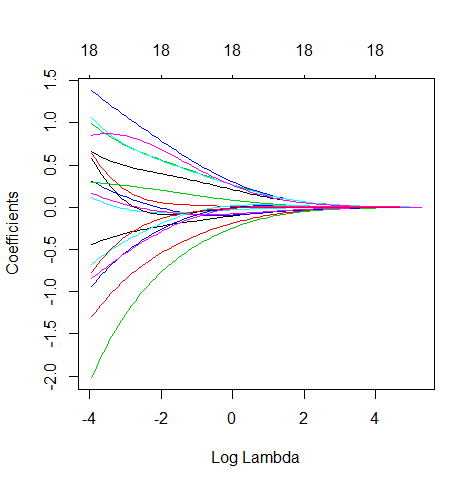
\includegraphics[scale=0.3]{images/ridge_coefficients_path}
		\caption{Ridge ($\alpha=0$)}
		\label{fig:glm-path-ridge}
	\end{subfigure}
	\hfill
	\begin{subfigure}[b]{0.3\textwidth}
		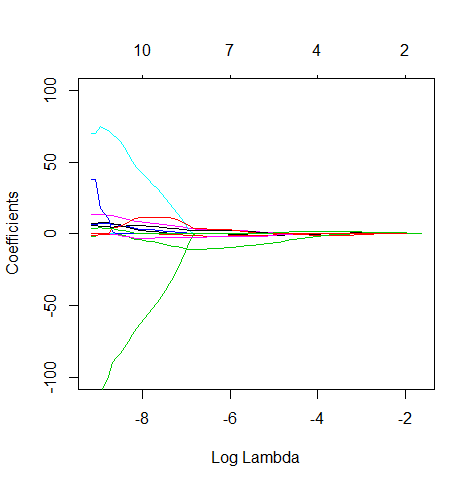
\includegraphics[scale=0.3]{images/lasso_coefficients_path}
		\caption{Lasso ($\alpha=1$)}
		\label{fig:glm-path-lasso}
	\end{subfigure}
	\hfill
	\begin{subfigure}[b]{0.3\textwidth}
		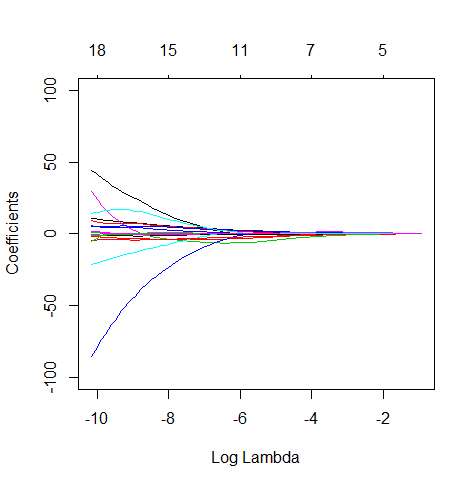
\includegraphics[scale=0.3]{images/elastic_coefficients_path}
		\caption{Elastic net ($\alpha=0.5$)}
		\label{fig:glm-path-elastic}
	\end{subfigure}
	\caption{Co\"effici\"ent paths as a function of $\lambda$ for different regularization types.}
	\label{fig:glm-paths}
\end{figure}

\subsection{Lambda}
\label{subsec:glm-lambda}
Using a regularizer introduces a constraint, this means that we now have to deal with a constrained optimization problem which is much harder to solve than an unconstrained problem. Fortunately, through some clever mathematics it is possible to convert the constrained minimization problem to an unconstrained one by incorporating the regularization constraint in the formula for the error itself\cite{caltechmachinelearning}. The formula for the error with regularization then becomes:
$$
E_{in}(w) = \frac{1}{N}\sum_{n=1}^{N}e(x_{n},y_{n},w)+\lambda R(w)
$$
where
\begin{itemize}
	\item $E_{in}(w)$ is the in-sample error.
	\item $e(x_{n},y_{n},w)$ is the individual error made on example n. In the case of logistic regression this would be a cross-entropy error term $ln(1+e^{-y_{n}w^{T}x_{n}})$.
	\item $\lambda$ is the regularization parameter that will be explained below.
	\item $R(w)$ is the regularization term dependent on the type of regularization used. For instance: $\sum_{i=1}^{N}\lvert w_{i}\rvert$ for lasso, $\sum_{i=1}^{N}w_{i}^{2}$ for ridge, ...
	\item $x_{n}$ is the n'th sample in the dataset.
	\item $y_{n}$ is the outcome for the n'th sample in the dataset.
	\item $w$ is the vector of weights, our model parameters that we are trying to find.
\end{itemize}
Notice that we now again have an error measure that we want to minimize, and it is an unconstrained optimization problem. The important new part is $\lambda$. This is the amount of regularization we want to use. It is a new form for the constraint constant $C$ that was earlier introduced in the types of regularization. The higher $\lambda$ the tighter the constraint (lower $C$) and vice versa. The value of $\lambda$ will prove to be critical in getting good models. The way to calculate it is through validation.
\section{Validation}
\label{sec:glm-validation}
In this section we will explain the method of validation which is used to estimate the out-of-sample error. We will first explain the issue of sample size and then present a method to work around this limitation.
\subsection{The sample size dilemma}
Remember that when we are training a model we use the in-sample error to navigate the hypothesis space. We do this because we believe that the in-sample error is a valid surrogate for the out-of-sample error (which is the error we actually want to minimize).
A valid question to ask is: why don't we just estimate the out-of-sample error and minimize it directly? Consider the following situation: \\
We are given a dataset of $N$ samples. We will use $K$ samples of the dataset to train my model, this leaves me with $N-K$ samples that are not used for training. Since $K$ samples were used for training, if we would compute the error the model makes on these samples we would be computing the in-sample error. If we want to estimate the out-of-sample error we have to use the $N-K$ samples that were not used for training. This sample set of $N-K$ samples if often called the validation set.\\
We can now make the following observations:
\begin{itemize}
	\item The larger we choose K, the more samples are available for training and thus the better our model can be (due to lower variance!)
	\item The larger we choose K, the less accurate our out-of-sample error estimate is, because we have fewer datapoints for the estimation
\end{itemize}
So now it is clear that we have a tradeoff to make. We would like K to be as large as possible so that we have a large amount of samples to train a model from. On the other hand we would like K to be as small as possible so that we have enough samples to estimate the out-of-sample error. The solution to this apparent contradiction will be cross-validation.
\subsection{Cross-validation}
Cross-validation\cite{caltechmachinelearning}\cite{kohavi1995study} is a technique that allows us to have plenty of samples left for training, while still getting a pretty good estimate for the out-of-sample error. The method is as follows: divide the dataset of $N$ samples into $F$ equal parts (often called folds). Each fold now has $N/F$ samples. Train a model on $F-1$ folds and use the remaining fold to estimate the out-of-sample error. Repeat this process $F$ times, one time for each of the $F$ folds, each time leaving out a different fold. In the end we have $F$ estimates of the out-of-sample error and we can average them to get a final result.\\ \\
Notice that we are really using all samples for validation and training, but never both at the same time. It feels a bit like cheating, but in practice this method works wonderfully. Validation is often used to determine parameters of the learning process, for instance the $\lambda$ parameter for regularization. We simply try several values for $\lambda$, compute the out-of-sample error using validation, and pick the $\lambda$ that gives the lowest error. Once we have decided this $\lambda$ we can then train a model on the full dataset of $N$ points and use the $\lambda$ we have just calculated to be optimal. \\ \\
We have to remark however that when we use validation to calculate a value for $\lambda$ as described above, we are really using the validation to help train the model. In this case we can no longer make the statement that the validation samples are not used for training. This is called data pollution. We are using the same data to train training parameters aswell as training the model itself and it is obvious that this will give rise to additional correlations in the data. However in practice it is generally accepted that if you use this technique to decide on just a few learning parameters (often just $\lambda$), and you have a big enough dataset, the data pollution is minimal and the results and estimates you get are still reliable\cite{caltechmachinelearning}. \\ \\

Cross-validation is not only used to estimate learning parameters. It can also be used to test the performance of the model. In this case the fold that is not used for training is usually not called a validation set, but rather a test set. Because samples in this set will be used to test the models performance. 

\section{Conclusion}
\label{sec:glm-conclusion}
We have now covered the basis of Generalized Linear Models. We have described the gradient descent method that we can use to navigate the hypothesis space by minimizing an error function. We have seen that overfitting is a serious issue that is caused by noise at different levels of the learning process. We have broken down this noise into bias and variance and shown that we can have an impact on this process. We can use regularization to add a slight bias in order to greatly decrease the error due to variance and we have based this on the principle that we should prefer simple and smooth models. Lastly we have covered the method of validation. A method that we can use to estimate the out-of-sample error and which gives us the ability to choose learning parameters like $\lambda$ and also test the performance of our model.

%%% Local Variables: 
%%% mode: latex
%%% TeX-master: "thesis"
%%% End: 
